\documentclass{article}
\usepackage{graphics} % for pdf, bitmapped graphics files
\usepackage{graphicx} % for pdf, bitmapped graphics files
\usepackage{epsfig} % for postscript graphics files
\begin{document}


\section{What is WikiModel?}
\begin{itemize}
 \item WikiModel is a Data Model defining the structure of wiki documents\begin{itemize}
 \item Defines wiki document elements and rules of their possible imbrications (like DTD/Schema for XML documents)
\end{itemize}

 \item WikiModel is an API providing access to the structure of wiki documents\begin{itemize}
 \item This API gives access to and control over the internal structure of individual wiki documents
 \item Usage of this API guaranties that the accessed wiki documents respect the structure defined by the model
 
\end{itemize}

\end{itemize}

\section{What WikiModel isn't?}
\begin{itemize}
 \item It is not a Wiki Engine
 \item It does not work with a data storage, versioning, access rights,...
 \item It does not check or validate references between documents
\end{itemize}

\section{How can WikiModel be used?}
\begin{itemize}
 \item As a rendering engine to transform various wiki  syntaxes to formatted content (HTML, PDF, TeX, ...)
 \item As a parser for semantic annotations
\end{itemize}

\section{How WikiModel Works?}

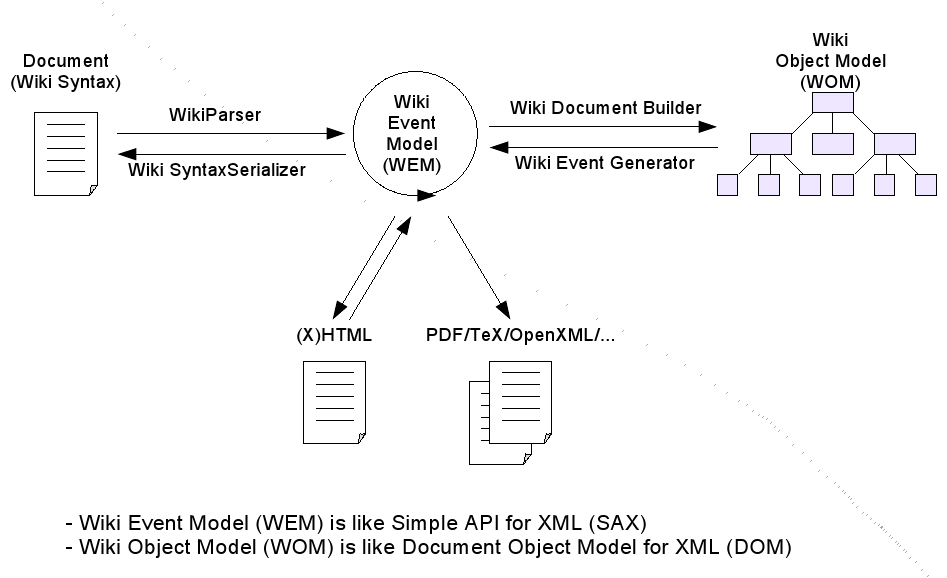
\includegraphics[bb=0 0 300 183]{HowWikiModelWorks.png}


\section{WikiModel v1}

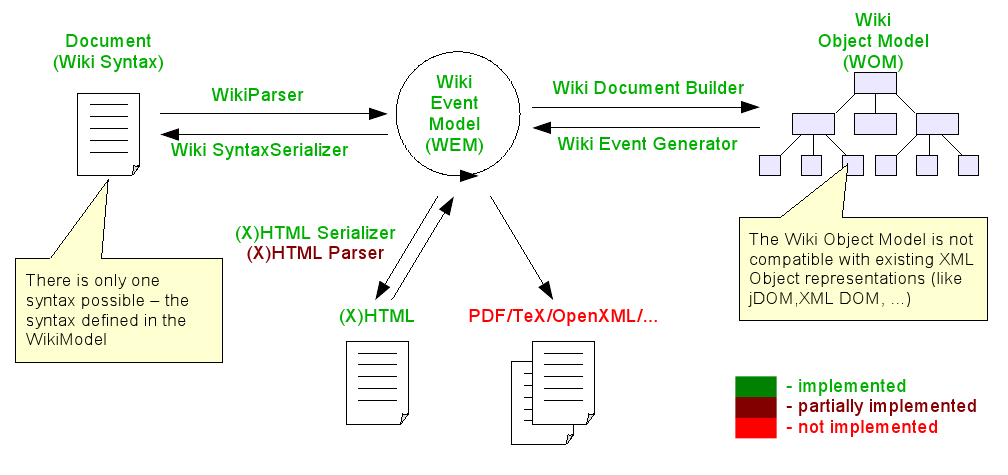
\includegraphics[bb=0 0 300 141]{WikiModel_v1.png}


\section{WikiModel v2}

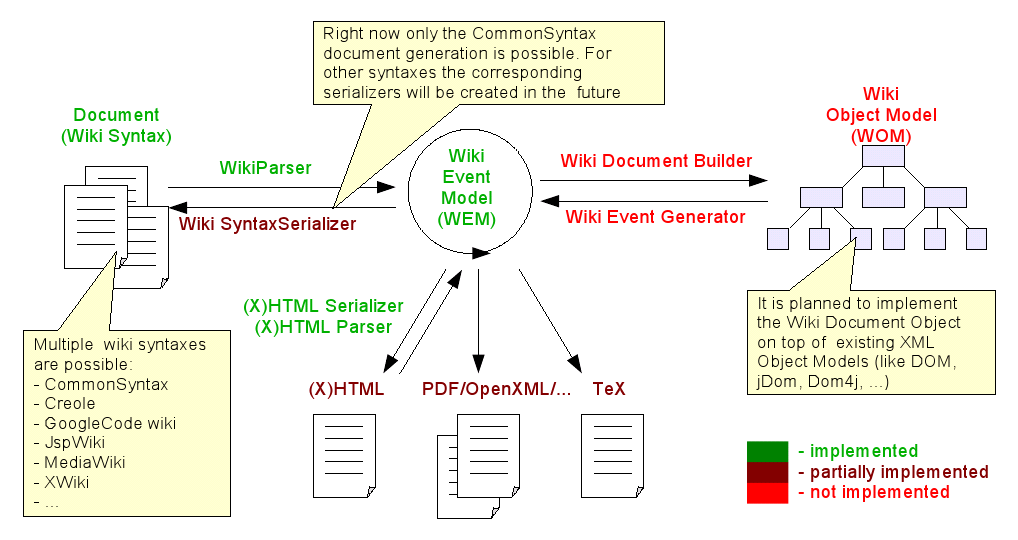
\includegraphics[bb=0 0 300 159]{WikiModel_v2.png}


\section{WikiModel v1 and v2: Comparision}

\subsection{WikiModel v1}
\begin{itemize}
 \item Exists only one WikiModel-specific  syntax 
 \item Real grammar based parser (JavaCC)
 \item Possibility to work with “embedded” documents
 \item Semantic statements about documents 
\end{itemize}

\subsection{WikiModel v2 }
\begin{itemize}
 \item Keeps all the features of v1 +
 \item All parsers much faster than v1
 \item CommonSyntax manipulates with greater number of structural elements than in v1
 \item Possibilities to work with documents written with multiple syntaxes
 \item All parsers are based on real JavaCC grammars
 \item Possibility to work with “embedded” documents
 \item Semantic statements about parts of the text  
\end{itemize}

\section{How WikiParser (v2) works}

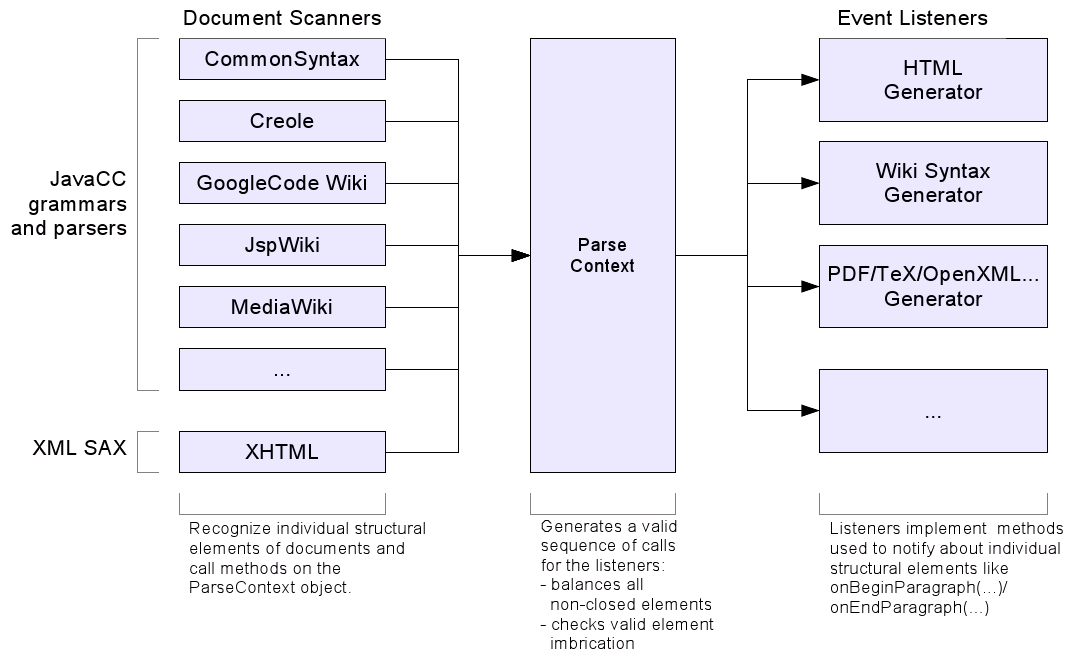
\includegraphics[bb=0 0 300 183]{HowWikiParserV2Works.png}


\section{Features of WikiModel v2}
\begin{itemize}
 \item WikiModel itself does not depend on any particular wiki syntax\begin{itemize}
 \item WikiModel manipulates with a fixed number of structural element types and defines their possible assembly/imbrication
 \item Simplified structure (relative to XHTML)  greatly simplifies the validation and manipulation of documents
 \item The document schema is sufficiently flexible to simulate almost any HTML formatting (like tables with embedded lists, headers and paragraphs)
 \item This is a super-set of structural elements existing in others wikies, so the information from any wiki can be imported without loosing the information or structure
\end{itemize}

 \item Contains notions of semantic statements about the  documents and parts of a document
 \item CommonSyntax manipulates with all possible structural elements defined by the WikiModel v2
 \item Parsers for multiple wiki syntaxes are available (JspWiki, XWiki, MediaWiki, Creole, GoogleCode wiki, ...). \begin{itemize}
 \item All parsers give access to the valid structure of documents. If a document contains non-valid elements (non-closed markup or overlapping elements) then it will be fixed automatically
\end{itemize}

\end{itemize}

\section{CommonSyntax: Example}

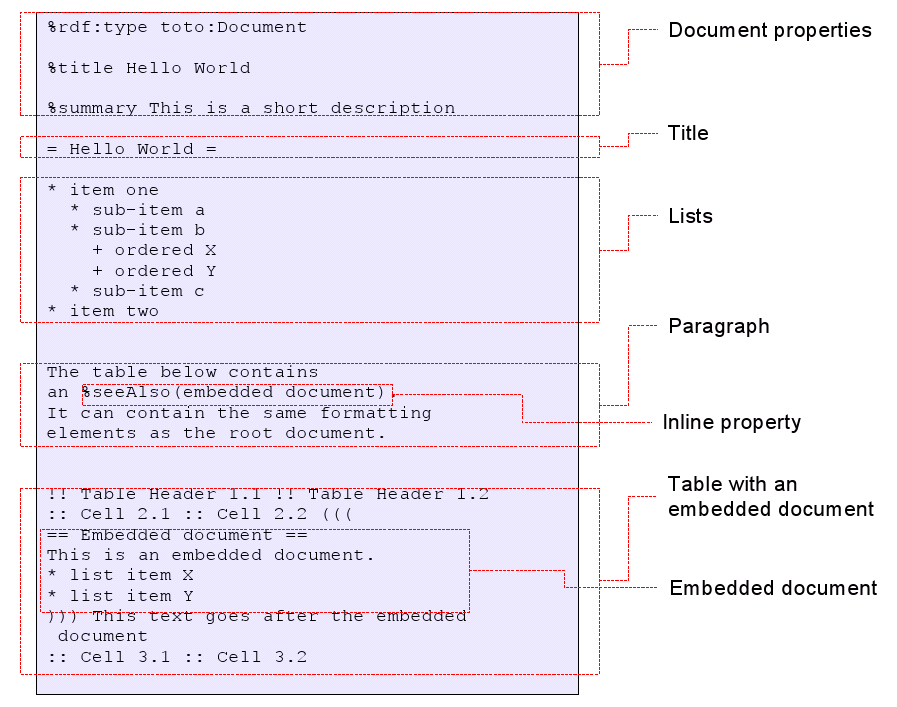
\includegraphics[bb=0 0 300 236]{CommonSyntaxExample1.png}


\section{CommonSyntax: How it can be used}

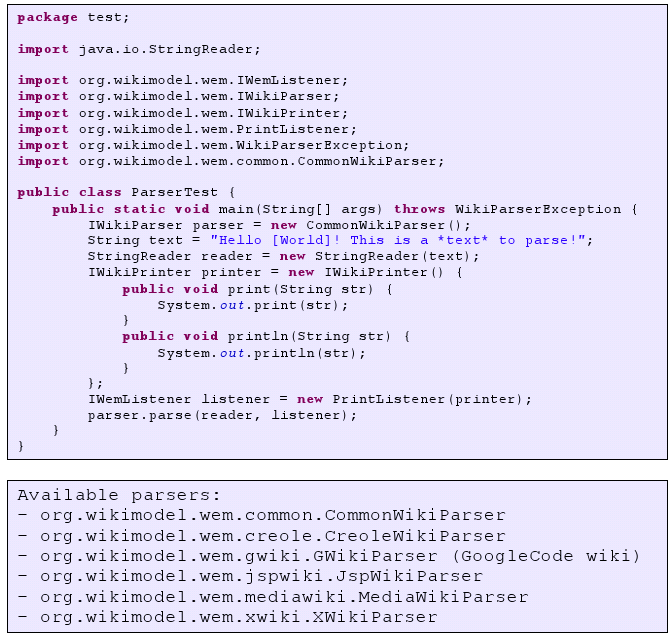
\includegraphics[bb=0 0 300 285]{CommonSyntaxExample2.png}

\end{document}
